\documentclass{article}

%other packages
\usepackage[a4paper]{geometry}
\usepackage{longtable}
\usepackage{wrapfig}
\setlength\parindent{0pt}
\usepackage{enumitem}
\usepackage[table]{xcolor}
\usepackage{polynom}
\def\scaleint#1{\vcenter{\hbox{\scaleto[3ex]{\displaystyle\int}{#1}}}}
\usepackage{array}
\newcolumntype{C}{>{{}}c<{{}}} % for '+' and '-' symbols
\newcolumntype{R}{>{\displaystyle}r} % automatic display-style math mode 
\usepackage{tabularray}
\usepackage{dcolumn,tabularx,booktabs}

%maths
\usepackage{mathtools}
\usepackage{amsmath}
\usepackage{amssymb}
\usepackage{amsfonts}
\usepackage{autobreak}

%tikzpicture
\usepackage{tikz}
\usepackage{scalerel}
\usepackage{pict2e}
\usepackage{tkz-euclide}
\usepackage{tikz-3dplot}
\usetikzlibrary{calc}
\usetikzlibrary{patterns,arrows.meta}
\usetikzlibrary{shadows}
\usetikzlibrary{external}
\usetikzlibrary{decorations.pathreplacing,angles,quotes}

%pgfplots
\usepackage{pgfplots}
\pgfplotsset{compat=1.18}
\usepgfplotslibrary{statistics}
\usepgfplotslibrary{fillbetween}

\pgfplotsset{
    standard/.style={
    axis line style = thick,
    trig format=rad,
    enlargelimits,
    axis x line=middle,
    axis y line=middle,
    enlarge x limits=0.15,
    enlarge y limits=0.15,
    every axis x label/.style={at={(current axis.right of origin)},anchor=north west},
    every axis y label/.style={at={(current axis.above origin)},anchor=south east}
    }
}

\begin{document}

\begin{center}
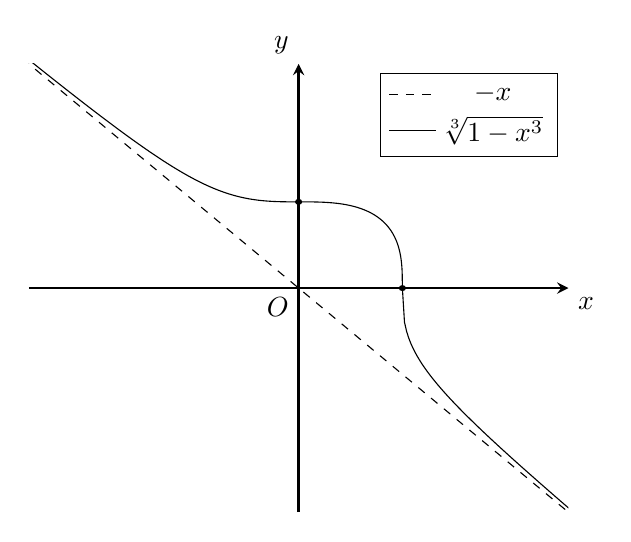
\begin{tikzpicture}
\begin{axis}[
standard,
xmin=-2, xmax=2,
ymin=-2, ymax=2,
xtick={\empty}, ytick={\empty},
xlabel={$x$}, ylabel={$y$}]
\addplot[dashed]{-x};\addlegendentry{\(-x\)}
\addplot[samples=100,domain=-3:0]{-x*(1-1/x^3)^(1/3)};
\addplot[samples=500,domain=0:1]{(1-x^3)^(1/3)};\addlegendentry{\(\sqrt[3]{1-x^3}\)}
\addplot[samples=100,domain=1:3]{-x*(1-1/x^3)^(1/3)};
\node[below left] at (0,0) {$O$};
\fill (0,1) circle [radius=0.035];
\fill (1,0) circle [radius=0.035];
\end{axis}
\end{tikzpicture}
\end{center}

\end{document}